\thispagestyle{plain}
\section{Ecuaciones cuadráticas}
\boxabstract{Aprendizajes esperados:}{Resuelve problemas mediante la formulación y la solución algebraica de ecuaciones cuadráticas.}
\subsection{Ecuaciones cuadráticas}

Analiza las situaciones y contesta lo que se pide.\\

\begin{boxK}
    \begin{center}\textbf{Inicio}\end{center}
    Lee la situación, observa la imagen y responde lo que se pide.
    \begin{enumerate}
        \item Martín fue contratado para cercar un terreno con 120 m de malla. Le pidió a su cliente
              los datos del terreno, quien se los entregó en un papel. Al llegar a su casa, Martín se dio
              cuenta de que perdió la información y sólo recordó que el triple del ancho menos el
              largo es igual a 28 m. No quiso llamar nuevamente al cliente y determinó las dimensio-
              nes del terreno. \textbf{¿Cuáles son?}
              \begin{enumerate}
                  \item Asigna variables y escribe las ecuaciones que modelan la situación.
                  \item Describe un procedimiento para resolverlas.
                  \item Determina las medidas de los lados del terreno.
                  \item ¿Qué información es relevante para responder y
                        cuál no?
                  \item Describe tu procedimiento para saber las respuestas.
              \end{enumerate}
    \end{enumerate}

\end{boxK}

\begin{enumerate}
    \item El hotel \emph{El Sol} gestionó con el municipio tener una zona de nado en el mar
          para el disfrute de sus huéspedes. Le han asignado 600 m$^2$ de superficie
          de mar y debe delimitarla con una cuerda y boyas para seguridad de los
          bañistas. El gerente del hotel quiere que la zona sea cuadrada, \\
          \textbf{¿cuál es la longitud de los lados? (figura \ref{fig:square})}.

          \begin{minipage}{.45\textwidth}
              \begin{figure}[H]
                  \centering
                  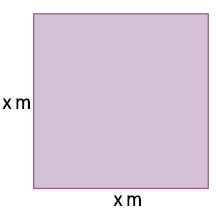
\includegraphics[width=0.4\linewidth]{square.png}
                  \captionof{figure}{Modelo geométrico de la situación.}
                  \label{fig:square}
              \end{figure}%
          \end{minipage}\hfill
          \begin{minipage}{.45\textwidth}
              \begin{figure}[H]
                  \centering
                  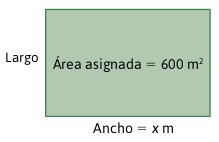
\includegraphics[width=0.6\linewidth]{square2.png}
                  \captionof{figure}{Modelo geométrico de la situación.}
                  \label{fig:square2}
              \end{figure}
          \end{minipage}

          \begin{enumerate}
              \item ¿Cuáles son las cantidades conocidas?
              \item ¿Cuáles son las cantidades desconocidas?
              \item Escriban una ecuación que modele la situación.
              \item ¿Cuál es la longitud de los lados?
          \end{enumerate}

    \item Antes de que se hiciera la delimitación de la zona de nado, el gerente del
          hotel cambió de opinión acerca de la forma de esta zona. Ahora debía
          ser rectangular con cierta característica: el largo tiene 10 m menos que
          el ancho. \textbf{¿Cuál es la longitud de los lados de la superficie delimitada?
              (figura \ref{fig:square2})}.\\
          \begin{enumerate}
              \item ¿Cuáles son las cantidades conocidas?
              \item ¿Cuáles son las cantidades desconocidas?
              \item Escriban una ecuación que modele la situación.
              \item Planteen una forma de resolver el problema. ¿Cuál es la longitud de los
                    lados?
          \end{enumerate}

          \begin{boxH}
              Una \textbf{ecuación cuadrática} completa en una variable es una ecuación del tipo
              \begin{equation}
                  ax^2 + bx + c = 0
              \end{equation}
              donde $a$, $b$ y $c$ son enteros, decimales o fraccionarios y $a$ no es igual a 0. Como el
              mayor exponente de la variable es 2 también se
              le conoce como \textbf{ecuación de segundo grado}.
          \end{boxH}

    \item Considera el problema anterior. El municipio ha
          notificado al gerente del hotel El Sol que hubo un error en la asignación de la zona
          de mar y que en lugar de 600 m$^2$ , se le asignan 504 m$^2$ . El gerente del hotel aún
          quiere que la zona de nado tenga 10 m menos de largo que de ancho. \textbf{¿Cuál es la
              nueva longitud de los lados?}

          \begin{enumerate}
              \item Identifiquen las cantidades conocidas, desconocidas y escriban una ecuación que
                    modele la situación.
              \item Verifiquen cuáles valores son soluciones o raíces de la ecuación anterior y escriban
                    por qué.
                    \begin{itemize}
                        \item $x = -28$.
                        \item $x = -18$.
                        \item $x = -8$.
                        \item $x = 0$.
                        \item $x = 8$.
                        \item $x = 18$.
                        \item $x = 28$.
                    \end{itemize}

          \end{enumerate}
          \begin{boxH}
              Un número que satisface una ecuación, es decir, que al sustituirlo en la variable de
              la ecuación se cumple la igualdad es llamado \textbf{solución} o \textbf{raíz} de la ecuación.
          \end{boxH}

          \newpage

    \item Completa la tabla \ref{tab:table01} sustituyendo los valores de x en cada expresión y haciendo las operaciones, luego respondan lo que se pide.

          \begin{figure}[H]
              \centering
              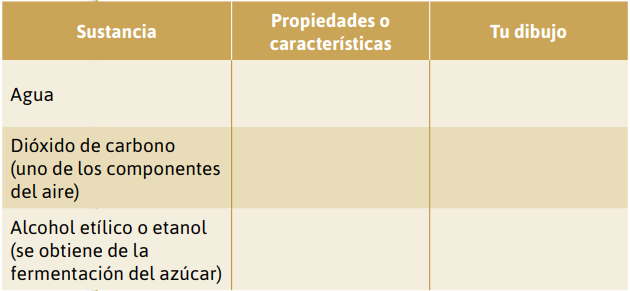
\includegraphics[width=0.8\textwidth]{tabla01.png}
              \captionof{figure}{Modelo geométrico de la situación.}
              \label{tab:table01}
          \end{figure}

          \begin{enumerate}
              \item ¿Cómo son los valores de las tres expresiones? ¿Qué pueden concluir sobre ellas?
              \item ¿Cómo pueden saber que un producto de expresiones algebraicas es equivalente a una ecuación de segundo grado?
          \end{enumerate}


    \item Se tienen dos expresiones algebraicas: $(x - 1)(x - 6) = 0$ y $x^2 - 7x + 6 = 0$.

          \begin{enumerate}
              \item ¿Cuál es una ecuación cuadrática? ¿Por qué?
              \item ¿Cuántas soluciones tiene la ecuación (x - 1)(x - 6) = 0? Explica.
              \item ¿Cuántas soluciones tendrá la ecuación x$^2 - 7x + 6 = 0$? ¿Por qué?
              \item ¿Cuántas soluciones tendrá una ecuación cuadrática?
                    Analicen los siguientes casos:
                    \[(x)(x) = 1 \text{\quad y \quad} x^2 = 1\]
                    \[x(x - 1) = 0 \text{\quad y \quad}x^2 - x = 0\]
                    \[(x - 1)(x - 2) = 0 \text{\quad y \quad} x^2 - 3x + 2 = 0\]
                    \[(x - 1)(x - 2) + 1 = 0 \text{\quad y \quad} x^2 - 3x + 3 = 0\]
                    Comprueben primero que cada par de ecuaciones es equivalente. Pueden probar por ensayo y error para
                    encontrar las soluciones.\\
          \end{enumerate}
\end{enumerate}

\begin{boxK}
    \begin{center}\textbf{Cierre}\end{center}

    \begin{minipage}[t]{0.2\textwidth}
        \begin{figure}[H]
            \centering
            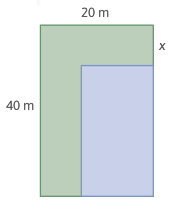
\includegraphics[width=\linewidth]{s7l1_cierre.png}
            \captionof{figure}{Modelo geométrico de la situación.}
            \label{fig:s7l1_cierre}
        \end{figure}
    \end{minipage}\hfill
    \begin{minipage}[t]{0.8\textwidth}
        \begin{enumerate}
            \item Retoma la situación de la actividad de inicio y responde, completa o corrige
                  tus respuestas. ¿Qué pasaría con las soluciones de la ecuación si los 120 son
                  metros cuadrados?
                  Reflexiona acerca de los conocimientos o las habilidades que necesitabas al
                  inicio y que ahora has adquirido. Escribe en tu cuaderno una conclusión.
            \item Los desarrolladores de un fraccionamiento habían planeado que algunos
                  terrenos para construir las casas fueran de 20 por 40 metros, pero los
                  40 m
                  reducirán de tal manera que tengan 525 m$^2$ de área para ampliar los adadores, como se muestra en la figura \ref{fig:s7l1_cierre}.
                  \begin{enumerate}
                      \item ¿De cuánto será el ancho del camino?
                      \item ¿Cómo planteas la ecuación que permite resolver el problema?
                  \end{enumerate}
        \end{enumerate}
    \end{minipage}


\end{boxK}

\newpage

\subsection{Gr\'aficas de expresiones cuadráticas y soluciones de sus ecuaciones}
\begin{boxK}
    \begin{center}\textbf{Inicio}\end{center}
    \begin{enumerate}
        \item Lee la situación, observa la imagen y responde lo que se pide.
              La torre Eiffel tiene una altura de 324 m. Desde la parte superior se deja caer una pelota
              de golf. La gráfica que se muestra es la representación de la ecuación que describe este
              movimiento, sin considerar la resistencia del aire. \\
              \textbf{¿Cuánto tiempo tarda el objeto en llegar al suelo?}
              \begin{enumerate}
                  \item ¿Qué parte de la gráfica tiene sentido considerar?
                  \item ¿Qué altura corresponde al tiempo 0 s? ¿A qué tiempo corresponde la altura 0 m?
                  \item ¿Qué valor es la solución del problema? Explica.
                  \item ¿Qué significa en la situación el valor simétrico, es decir, de signo contrario, al que obtuviste en la pregunta anterior?
                  \item ¿Qué información es relevante para responder y cuál no?
                  \item Describe el procedimiento que realizaste para saber las respuestas.
              \end{enumerate}
        \item  Reúnanse en equipo. Comparen sus respuestas, argumenten. Corrijan si es necesario.
              Reflexionen sobre el uso de gráficas para describir y resolver ecuaciones.
              \begin{figure}[H]
                  \centering
                  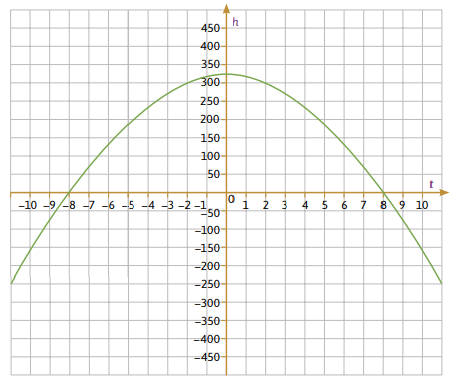
\includegraphics[width=0.65\textwidth]{parabole01.png}
                  \captionof{figure}{Modelo geométrico de la situación.}
                  \label{fig:parabole01}
              \end{figure}

    \end{enumerate}
\end{boxK}

\newpage

\subsubsection{Soluciones de ecuaciones cuadráticas con gráficas}

Analizaremos diversas gráficas de variaciones cuadráticas para determinar
la relación entre éstas y las soluciones de la ecuación asociada.

\begin{enumerate}
    \item Responde a los siguientes incisos.
          \begin{enumerate}

              \begin{minipage}[t]{0.3\textwidth}
                  \begin{figure}[H]
                      \centering
                      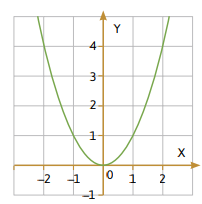
\includegraphics[width=\linewidth]{parabole02.png}
                      \captionof{figure}{Gráfica de $y = x^2$}
                      \label{fig:parabole02}
                  \end{figure}
              \end{minipage}\hfill
              \begin{minipage}[t]{0.6\textwidth}
                  \item Analicen la gráfica de $y = x^2$ (figura \ref{fig:parabole02}).
                  \begin{enumerate}
                      \item Localiza los puntos en los que la gráfica interseca al eje X. ¿Cuál
                            es el valor de $x$ en esos puntos?
                      \item Sustituye esos valores en la ecuación $x^2= 0$. ¿Qué observas?
                      \item Elije otros dos puntos que estén sobre la gráfica. ¿Cuál es el valor de $x$ en esos puntos?
                      \item Sustituyan esos nuevos valores en la ecuación $x^2= 0$. ¿Qué observas?
                  \end{enumerate}
              \end{minipage}

              \begin{minipage}[t]{0.6\textwidth}
                  \item Analiza la gráfica de $y = x - 1$ (figura \ref{fig:parabole03}) y responde.
                  \begin{enumerate}
                      \item Localiza los puntos en los que la gráfica interseca al eje X. ¿Cuál es el valor de $x$ en esos puntos?
                      \item Elije otros dos puntos que estén sobre la gráfica. ¿Cuál es el valor de $x$ en esos puntos?
                      \item Sustituye esos nuevos valores en la ecuación $x^2 - 1 = 0$. ¿Qué observas?
                      \item ¿Qué puedes decir acerca de las soluciones de la ecuación $x^2 - 1 = 0$?
                  \end{enumerate}
              \end{minipage}\hfill
              \begin{minipage}[t]{0.3\textwidth}
                  \begin{figure}[H]
                      \centering
                      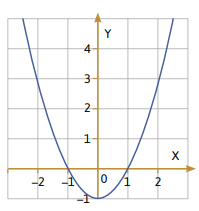
\includegraphics[width=\linewidth]{parabole03.png}
                      \captionof{figure}{Gráfica de $y = x^2 - 1$}
                      \label{fig:parabole03}
                  \end{figure}
              \end{minipage}

              \begin{minipage}[t]{0.3\textwidth}
                  \begin{figure}[H]
                      \centering
                      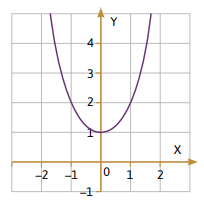
\includegraphics[width=\linewidth]{parabole04.png}
                      \captionof{figure}{Gráfica de $y = x^2 + 1$.}
                      \label{fig:parabole04}
                  \end{figure}
              \end{minipage}\hfill
              \begin{minipage}[t]{0.6\textwidth}
                  \item Analicen la gráfica de $y = x^2 + 1$  (figura \ref{fig:parabole04}).
                  \begin{enumerate}
                      \item Localiza los puntos en los que la gráfica interseca al eje X. ¿Cuál
                            es el valor de $x$ en esos puntos?
                      \item Elije otros dos puntos que estén sobre la gráfica. ¿Cuál es el valor de $x$ en esos puntos?
                      \item Sustituye esos nuevos valores en la ecuación $y = x^2 + 1$. ¿Qué observas?
                      \item ¿Qué puedes decir acerca de las soluciones de la ecuación $x^2 + 1 = 0$?
                  \end{enumerate}
              \end{minipage}
              ¿Qué semejanzas y diferencias observan entre las tres expresiones?
              ¿Y entre sus gráficas? Con base en las gráficas anteriores, ¿cuántas soluciones pue-
              de tener una ecuación cuadrática? ¿Cómo pueden determinar las soluciones?
          \end{enumerate}

          % \newpage

    \item Responde a los siguientes incisos.
          \begin{enumerate}

              \begin{minipage}[t]{0.3\textwidth}
                  \begin{figure}[H]
                      \centering
                      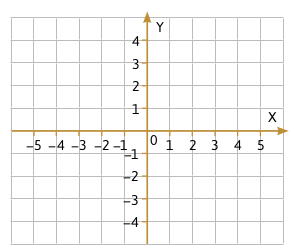
\includegraphics[width=\linewidth]{xyplane.png}
                      \captionof{figure}{}
                      \label{fig:xyplane}
                  \end{figure}
              \end{minipage}\hfill
              \begin{minipage}[t]{0.6\textwidth}
                  \item Considera la expresión $\frac{1}{2}x^2 + x$. Completa la tabla \ref{tab:table02} para
                  obtener algunos valores y con base en éstos realiza la gráfica en la figura \ref{fig:xyplane}.
                  Aproxima a un decimal.
                  \begin{figure}[H]
                      \centering
                      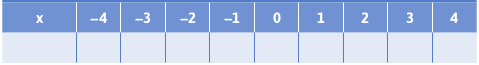
\includegraphics[width=0.9\linewidth]{tabla02.png}
                      \captionof{table}{}
                      \label{tab:table02}
                  \end{figure}
                  Con base en la gráfica, ¿cuántas soluciones tiene la ecuación $\frac{1}{2}x^2 + x= 0$? ¿Cuáles son?
              \end{minipage}

              \begin{minipage}[t]{0.6\textwidth}
                  \item Considera la expresión $\frac{1}{2}x^2 - x$. Completa la tabla \ref{tab:table03} para
                  obtener algunos valores y con base en éstos realiza la gráfica en la figura \ref{fig:xyplane2}.
                  Aproxima a un decimal.
                  \begin{figure}[H]
                      \centering
                      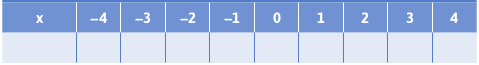
\includegraphics[width=0.9\linewidth]{tabla02.png}
                      \captionof{table}{}
                      \label{tab:table03}
                  \end{figure}
                  Con base en la gráfica, ¿cuántas soluciones tiene la ecuación $\frac{1}{2}x^2 - x= 0$? ¿Cuáles son?
              \end{minipage}\hfill
              \begin{minipage}[t]{0.3\textwidth}
                  \begin{figure}[H]
                      \centering
                      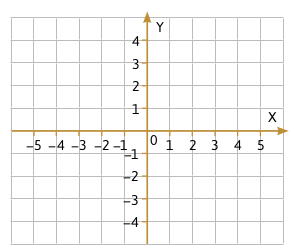
\includegraphics[width=\linewidth]{xyplane.png}
                      \captionof{figure}{}
                      \label{fig:xyplane2}
                  \end{figure}
              \end{minipage}

              \begin{minipage}[t]{0.3\textwidth}
                  \begin{figure}[H]
                      \centering
                      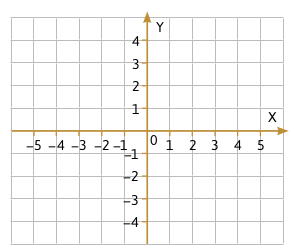
\includegraphics[width=\linewidth]{xyplane.png}
                      \captionof{figure}{}
                      \label{fig:xyplane3}
                  \end{figure}
              \end{minipage}\hfill
              \begin{minipage}[t]{0.6\textwidth}
                  \item Considera la expresión $-\frac{1}{2}x^2 + x$. Completa la tabla \ref{tab:table04} para
                  obtener algunos valores y con base en éstos realiza la gráfica en la figura \ref{fig:xyplane3}.
                  Aproxima a un decimal.
                  \begin{figure}[H]
                      \centering
                      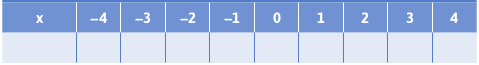
\includegraphics[width=0.9\linewidth]{tabla02.png}
                      \captionof{table}{}
                      \label{tab:table04}
                  \end{figure}
                  Con base en la gráfica, ¿cuántas soluciones tiene la ecuación $-\frac{1}{2}x^2 + x= 0$? ¿Cuáles son?
              \end{minipage}

              \begin{minipage}[t]{0.6\textwidth}
                  \item Considera la expresión $-\frac{1}{2}x^2 - x$. Completa la tabla \ref{tab:table05} para
                  obtener algunos valores y con base en éstos realiza la gráfica en la figura \ref{fig:xyplane4}.
                  Aproxima a un decimal.
                  \begin{figure}[H]
                      \centering
                      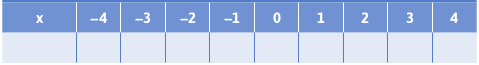
\includegraphics[width=0.9\linewidth]{tabla02.png}
                      \captionof{table}{}
                      \label{tab:table05}
                  \end{figure}
                  Con base en la gráfica, ¿cuántas soluciones tiene la ecuación $-\frac{1}{2}x^2 - x= 0$? ¿Cuáles son?
              \end{minipage}\hfill
              \begin{minipage}[t]{0.3\textwidth}
                  \begin{figure}[H]
                      \centering
                      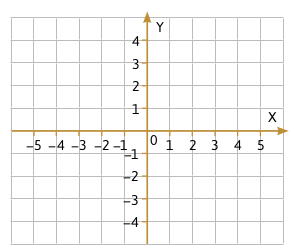
\includegraphics[width=\linewidth]{xyplane.png}
                      \captionof{figure}{}
                      \label{fig:xyplane4}
                  \end{figure}
              \end{minipage}
          \end{enumerate}
          ¿Qué semejanzas y diferencias observan entre las tres expresiones?
          ¿Y entre sus gráficas? Con base en las gráficas anteriores, ¿cuántas soluciones pue-
          de tener una ecuación cuadrática? ¿Cómo pueden determinar las soluciones?

          \begin{boxH}
              Las gráficas de expresiones cuadráticas pueden ser \emph{abiertas hacia arriba o hacia
                  abajo}. También pueden estar a la izquierda o derecha del origen.
              \begin{figure}[H]
                  \centering
                  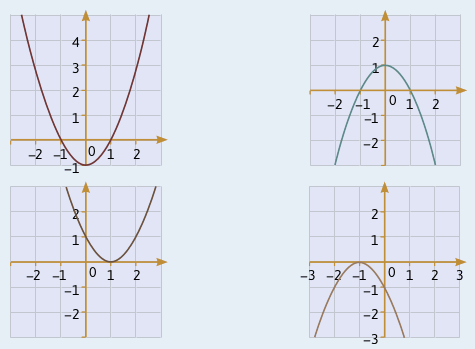
\includegraphics[width=\linewidth]{paraboles.png}
                  \captionof{figure}{}
                  \label{fig:paraboles}
              \end{figure}
          \end{boxH}

          \newpage

    \item Analiza las gráficas de la figura \ref{fig:paraboles2.6}. Determina el número
          de soluciones que tiene la ecuación en cada caso y escríbanlas.

          \begin{figure}[H]
              \centering
              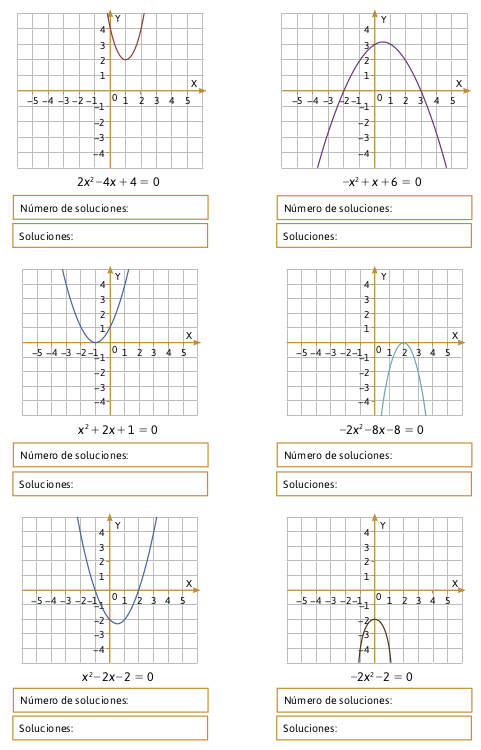
\includegraphics[width=0.8\linewidth]{paraboles2.6.png}
              \captionof{figure}{Gráficas de expresiones cuadráticas.}
              \label{fig:paraboles2.6}
          \end{figure}

          Con base en la gráfica de una expresión cuadrática de
          la forma $ax^2 + bx + c$, ¿cómo determinan el número de soluciones de la
          ecuación $ax^2 + bx + c = 0$? ¿Cómo determinan las soluciones? Escriban
          una conclusión en su cuaderno.
\end{enumerate}

\begin{boxK}
    \begin{center}\textbf{Cierre}\end{center}

    \begin{enumerate}
        \item Retoma la situación de la actividad de inicio y responde, completa o corrige
              tus respuestas. Si la gráfica abriera hacia arriba, ¿qué representaría?
              Reflexiona acerca de los conocimientos o las habilidades que necesitabas al
              inicio y que ahora has adquirido. Escribe en tu cuaderno una conclusión.
        \item María ha graficado la expresión $y = x^2-8x + 15$ para resolver las siguientes
              ecuaciones:
              \begin{itemize}
                  \item $x^2-8x + 15 = -2$
                  \item $x^2-8x + 15 = -1$
                  \item $x^2-8x + 15 = 0$
                  \item $x^2-8x + 15 = 1$
                  \item $x^2-8x + 15 = 2$
              \end{itemize}
              \begin{enumerate}
                  \item Traza las rectas que son paralelas al eje X y que pasan por $y = -2$, $y = -1$, $y = 0$, $y = 1$ y $y = 2$.
                  \item Localiza los puntos en los que interseca cada recta a la gráfica.
                  \item ¿Cuáles son los valores de $x$ de esos puntos?
                  \item Evalúa los valores obtenidos de cada intersección en su ecuación correspondiente. Por ejemplo, los valores obtenidos para la variable $x$ de la intersección de la recta que pasa por $y = 2$ y la gráfica en la ecuación $x^2 - 8x + 15 = 2$. ¿Qué observas?
                  \item ¿María puede resolver las ecuaciones con ayuda de la gráfica sin hacer operaciones? Explica.
              \end{enumerate}
    \end{enumerate}

    \begin{figure}[H]
        \centering
        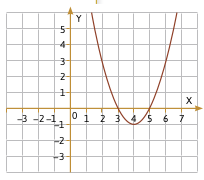
\includegraphics[width=0.4\linewidth]{s7l2_cierre.png}
        \captionof{figure}{}
        \label{fig:s7l2_cierre}
    \end{figure}
\end{boxK}

\begin{boxF}
    En un partido de campeonato, un futbolista patea el balón. Con
    base en la toma de una cámara, la computadora del centro de
    transmisión traza la trayectoria del balón y calcula la ecuación
    que la describe: $y = - \frac{1}{8}x^2 + 58 x + 74$ . Según la gráfica el futbolista
    está en el punto $x = -2$. ¿Hasta qué punto llegará la pelota?
    \begin{enumerate}
        \item ¿Qué parte de la gráfica tiene sentido según el problema?
        \item ¿Cuáles son las soluciones de la ecuación $-\frac{1}{8}x^2 + 58 x + 74 = 0$?
        \item ¿Qué significado tienen las soluciones dentro del problema?
        \item Si un jugador del equipo contrario que mida 1.80 m de altura
              se ubicara en $x = 0$, ¿taparía el disparo? Explica.
    \end{enumerate}

    \begin{figure}[H]
        \centering
        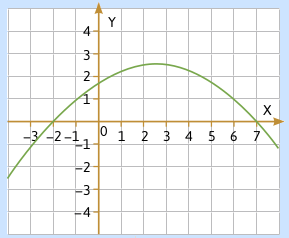
\includegraphics[width=0.4\linewidth]{futbolista.png}
        \captionof{figure}{Gráfica de la ecuación que representa la trayectoria del balón.}
        \label{fig:futbolista}
    \end{figure}
\end{boxF}

\newpage